\item \textbf{QuestionManager}:
	Il package \emph{QuestionManager} espone le funzionalità necessarie alla creazione e gestione di domande. Per permettere al package di essere estendibile in futuro con domande in diversi formati, le classi al suo interno sono organizzate seguendo il pattern \emph{Abstract Factory}. \\
	Il package contiene al suo interno le classi:
	\begin{itemize}
		\item \textit{QuestionFactory}
		\item \textit{Question}
		\item \textit{QML2HTMLFactory}
		\item \textit{HTMLQuestion}
		\item \textit{Translator}
	\end{itemize}
	
	\item\textbf{QuizManager}:
	Il Package \emph{QuizManager} espone le funzionalità necessarie alla creazione e gestione di quiz, collaborando con il package \emph{QuestionManager}. Per disaccoppiare la creazione di un quiz dalle domande che lo compongono, la classi all'interno del package seguono la struttura del design pattern \emph{Builder}.\\ 
	Il package contiene al suo interno le classi:
	\begin{itemize}
		\item \textit{QuizDirector}
		\item \textit{QuizBuilder}
		\item \textit{Quiz}
	\end{itemize}





\subsubsection{Package QuestionManager}	
Il package fa uso del design pattern \emph{Abstract Factory}.
\begin{figure}[h!]
\begin{center}
	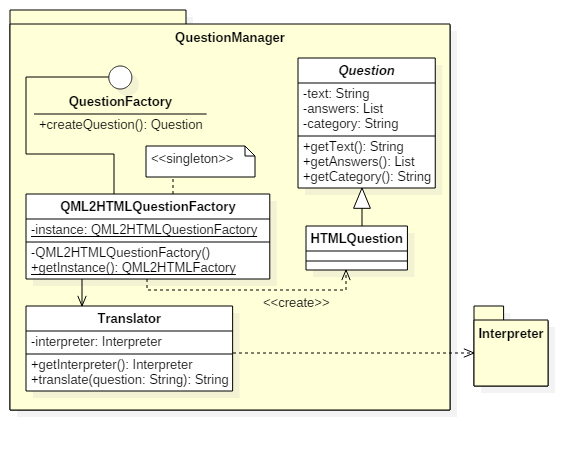
\includegraphics[scale=0.65]{../images/QuestionManagerClass.png}
	\caption{Diagramma delle classi del package QuestionManager}
\end{center}
\end{figure}
\subsubsubsection{Interfaccia QuestionFactory}
\begin{itemize}
	\item\textbf{Funzione del componente}: interfaccia di base delle Factory di tipi Question.
	\item\textbf{Relazione d'uso di altre componenti}: può essere concretizzata in diversi tipi di QuestionFactory.
	\item\textbf{Attività svolte e dati trattati}: definisce il contratto delle factory Question, cioè le operazioni di costruzione di Question che saranno definite in ogni concretizzazione.
\end{itemize}

\subsubsubsection{Classe astratta Question}
\begin{itemize}
	\item\textbf{Funzione del componente}: classe di base del tipo Question.
	\item\textbf{Relazione d'uso di altre componenti}: può essere concretizzata in diversi tipi di Question.
	\item\textbf{Attività svolte e dati trattati}: definisce il contratto generale delle Question, cioè le loro operazioni e dati.
\end{itemize}

\subsubsubsection{Classe QML2HTMLQuestionFactory}
La classe QML2HTMLQuestionFactory è un \emph{singleton}.
\begin{itemize}
	\item\textbf{Funzione del componente}: crea oggetti di tipo HTMLQuestion.
	\item\textbf{Relazione d'uso di altre componenti}: è concretizzazione della classe QuestionFactory. Crea oggetti HTMLQuestion. Si interfaccia con la classe Translator.
	\item\textbf{Attività svolte e dati trattati}: crea su richiesta oggetti di tipo HTMLQuestion, delegando la traduzione del codice QML alla classe Translator.
\end{itemize}

\subsubsubsection{Classe HTMLQuestion}	
\begin{itemize}
	\item\textbf{Funzione del componente}: rappresenta una domanda in formato HTML.
	\item\textbf{Relazione d'uso di altre componenti}: è concretizzazione di Question.
	\item\textbf{Attività svolte e dati trattati}: eredita e specializza le funzionalità dell'interfaccia Question.
\end{itemize}

\subsubsubsection{Classe Translator}
\begin{itemize}
	\item\textbf{Funzione del componente}: s'interfaccia con le componenti del package Interpreter per la traduzione di quesiti QML in HTML.
	\item\textbf{Relazione d'uso di altre componenti}: collabora con le interfacce Interpreter e InterpreterFactory.
	\item\textbf{Attività svolte e dati trattati}: riceve dalla classe ViewUpdater le richieste di traduzione e il codice QML da tradurre. Attraverso la factory InterpreterFactory (una sua concretizzazione) costruisce un Interpreter concreto e lo utilizza per la traduzione del codice. L'esito della traduzione viene reso disponibile a ViewUpdater.
\end{itemize}
\newpage

\subsubsection{Package QuizManager}
Il package fa uso del design pattern \emph{Builder}.
\begin{figure}[h!]
\begin{center}
	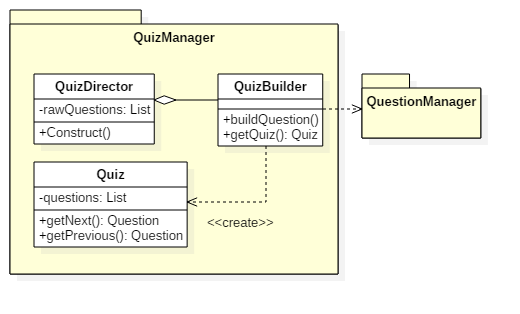
\includegraphics[scale=0.65]{../images/QuizManagerClass.png}
	\caption{Diagramma delle classi del package QuizManager}
\end{center}
\end{figure}
\subsubsubsection{Classe QuizDirector}
\begin{itemize}
\item\textbf{Funzione del componente}: è responsabile della costruzione di un oggetto di tipo Quiz.
	\item\textbf{Relazione d'uso di altre componenti}: utilizza la classe QuizBuilder.
	\item\textbf{Attività svolte e dati trattati}: la classe, a partire da un set di domande (in questo caso in QML), utilizza il Builder per costruire un Quiz.
\end{itemize}

\subsubsubsection{Classe QuizBuilder}
\begin{itemize}
\item\textbf{Funzione del componente}: Costruisce domanda per domanda un questionario.
	\item\textbf{Relazione d'uso di altre componenti}: interagisce con il package QuestionManager.
	\item\textbf{Attività svolte e dati trattati}: Costruisce passo pe r passo un oggetto di tipo Quiz. Si appoggia al package QuestionManager per la creazione delle singole domande.
\end{itemize}

\subsubsubsection{Classe Quiz}
\begin{itemize}
\item\textbf{Funzione del componente}: la classe rappresenta un Quiz, una raccolta di domande.
	\item\textbf{Relazione d'uso di altre componenti}: nessuna.
	\item\textbf{Attività svolte e dati trattati}: la classe possiede i dati e fornisce le operazioni necessaria alla fruizione di un Quiz.
\end{itemize}
\clearpage










\subsection{Builder}
	\begin{figure}[h!]
	\begin{center}
		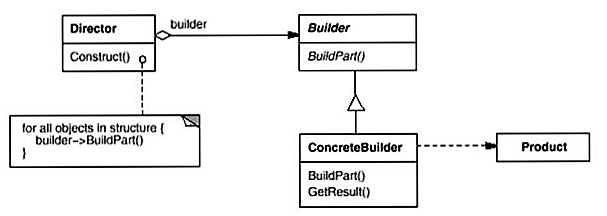
\includegraphics[scale=1]{../images/Builder.png}
		\caption{Design Pattern Builder}
	\end{center}
	\end{figure}
	\begin{itemize}
		\item\textbf{Scopo}: Separa la costruzione di un oggetto complesso dalla sua rappresentazione.
		\item\textbf{Applicabilità}:
		\begin{itemize}
			\item La procedura di creazione di un oggetto complesso
deve essere indipendente dalle parti che
compongono l'oggetto
			\item Il processo di costruzione deve permettere diverse
rappresentazioni per l'oggetto da costruire.
		\end{itemize}
		\item\textbf{Conseguenze}:
		\begin{itemize}
			\item Facilita le modifiche alla rappresentazione interna di
un prodotto
			\item Isola il codice dedicato alla costruzione di un prodotto
dalla sua rappresentazione
			\item Consente un controllo migliore del processo di
costruzione
		\end{itemize}
		\item\textbf{Utilizzo}: nel sistema Quizzipedia il design pattern è stato utilizzato nel package QuizManager per rendere la creazione di un Quiz indipendente dalle domande che lo compongono.
		\begin{figure}[h!]
	\begin{center}
		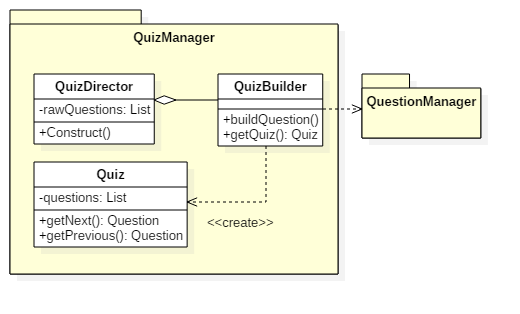
\includegraphics[scale=0.54]{../images/QuizManagerClass.png}
		\caption{Builder in QuizManager}
	\end{center}
	\end{figure}
	\end{itemize}
	\newpage
	
	
	\subsection{Command}
	\begin{figure}[h!]
	\begin{center}
		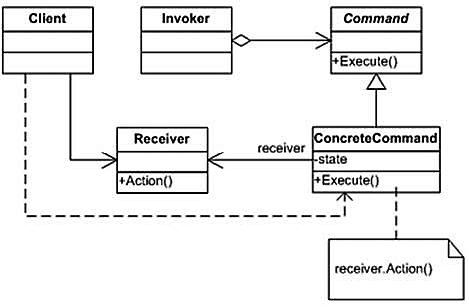
\includegraphics[scale=1]{../images/Command.png}
		\caption{Design Pattern Command}
	\end{center}
	\end{figure}
	\begin{itemize}
		\item\textbf{Scopo}: Incapsulare una richiesta in un oggetto, cosicché i
client sia indipendenti dalle richieste
		\item\textbf{Applicabilità}:
		\begin{itemize}
			\item Necessità di gestire richieste di cui non si conoscono i
particolari
			\item Parametrizzazione di oggetti sull'azione da eseguire
			\item Specificare, accodare ed eseguire richieste molteplici
volte
			\item Supporto ad operazioni di Undo e Redo e a transazioni.
		\end{itemize}
		\item\textbf{Conseguenze}:
		\begin{itemize}
			\item Accoppiamento "lasco" tra oggetto invocante e
quello che porta a termine l'operazione
			\item I command possono essere estesi
			\item I command possono essere composti e innestati
			\item È facile aggiungere nuovi comandi, le classi esistenti non devono essere modificate.
		\end{itemize}
		\item\textbf{Utilizzo}: nel sistema Quizzipedia il design pattern è stato utilizzato nel package Presenter, per disaccoppiare la ricezione degli input da parte della classe InputManager dalla loro risoluzione da parte di altre classi del Presenter e del Model. Il pattern permette inoltre di aggiungere facilmente nuovi \emph{Command} al sistema, estendendo l'interfaccia \emph{Input} del package UserInputManager. Sarà in questo modo più facile estendere le funzionalità offerte all'utente dal sistema Quizzipedia.
	\end{itemize}
	\begin{figure}[h!]
	\begin{center}
		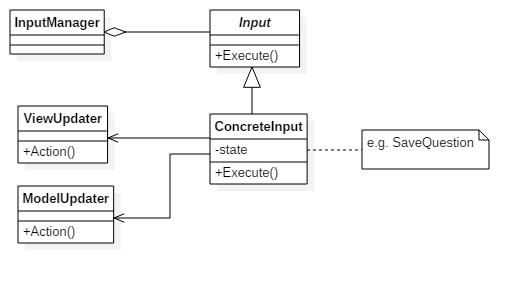
\includegraphics[scale=0.7]{../images/PresenterCommandDesignPattern.png}
		\caption{Design Pattern Command nel Presenter}
	\end{center}
	\end{figure}
	\newpage